
% Copyright (c) 2015 - 2019 Mario Mlačak, mmlacak@gmail.com
% Published as Public Domain work, under CC0 1.0 Universal Public Domain Dedication. See LICENSING, COPYING files for details.

% Classical Chess -----------------------------------------------------
\chapter*{Classical Chess}
\addcontentsline{toc}{chapter}{Classical Chess}
\label{ch:Classical Chess}

\begin{flushright}
\parbox{0.8\textwidth}{
\emph{A great war leaves the country with three armies -
an army of cripples, an army of mourners, and an army of thieves. \newline
\hspace*{\fill}{\textperiodcentered \textperiodcentered \textperiodcentered \hspace*{0.2em} German proverb} } }
\end{flushright}

\noindent
About Classical Chess is written really everything already, and I have
nothing to add, except to use it as an example on how to read the book.

\clearpage % ..........................................................
% Pieces **************************************************************

\section*{Pieces}
\addcontentsline{toc}{section}{Pieces}
\label{sec:Classical Chess/Pieces}

The easiest way to introduce readers to the rendering of classical pieces
is to show chessboard with initial setup:

\noindent
\begin{figure}[!h]
\includegraphics[width=1.0\textwidth, keepaspectratio=true]{boards/02_classical.png}
\caption{Classical Chess, initial setup}
\label{fig:02_classical}
\end{figure}

\noindent
You can compare this with official rendering at \algfmt{FIDE~2.3}.

\clearpage % ..........................................................

\subsection*{Bishop}
\addcontentsline{toc}{subsection}{Bishop}
\label{sec:Classical Chess/Pieces/Bishop}

\noindent
\begin{wrapfigure}[12]{l}{0.4\textwidth}
\centering
\includegraphics[width=0.4\textwidth, keepaspectratio=true]{pieces/bishop/02_classical.png}
\caption{Bishop}
\label{fig:bishop/02_classical}
\end{wrapfigure}
New pieces are introduced with zoomed-in image, on a \mbox{2 $\times$ 2} board.
Light pieces are rendered on a lower row, dark pieces are on an upper row,
regardless of actual colors used in a particular variant. % \newline
% \indent

Light fields are always in lower-right and upper-left corner, while dark fields
are always in lower-left and upper-right corner, regardless which actual colors
are used to paint board.

% ************************************************************** Pieces
% \clearpage % ..........................................................
% Chessboard **********************************************************

\section*{Chessboard}
\addcontentsline{toc}{section}{Chessboard}
\label{sec:Classical Chess/Chessboard}

As seen on the chessboard on previous page, light player starts from bottom of
a chessboard, while dark player starts from top. This arrangement is used by FIDE
(see \algfmt{FIDE~2.3}), and also for all examples in this book, and for all new
variants.

In such a setup, color of lower-right (and upper-left) corner are determined by
FIDE to be light colored, see \algfmt{FIDE~2.1}; this also applies to all new
variants, regardless which actual colors are used to paint chessboards.

In FIDE handbook, and elsewhere, chessboard is said to be made of \mbox{8 $\times$ 8}
grid of squares; in this book squares are referred to as fields.

\clearpage % ..........................................................
% Examples ============================================================

\subsection*{Examples}
\addcontentsline{toc}{subsection}{Examples}
\label{sec:Classical Chess/Chessboard/Examples}

\vspace*{-0.7\baselineskip}
\noindent
\begin{wrapfigure}[12]{l}{0.4\textwidth}
\centering
\includegraphics[width=0.4\textwidth, keepaspectratio=true]{examples/02_c/scn_cc_01_rook_not_blocked.png}
\vspace*{-1.4\baselineskip}
\caption{Rook not blocked}
\label{fig:scn_cc_01_rook_not_blocked}
\end{wrapfigure}
Some examples are not showing whole chessboard; often, those examples also
feature partial fields around sides to convey which part of chessboard has
been depicted. \newline
\indent
Here, we have hints of fields upwards and to the right, so example shows
lower-left corner of a chessboard. \newline
\indent
Green arrow is used in cases where move is legal, but there is nothing special
about it.

\vspace*{2.7\baselineskip}
\noindent
\begin{wrapfigure}[14]{l}{0.4\textwidth}
\centering
\includegraphics[width=0.4\textwidth, keepaspectratio=true]{examples/02_c/scn_cc_02_rook_blocked.png}
\vspace*{-1.4\baselineskip}
\caption{Rook blocked}
\label{fig:scn_cc_02_rook_blocked}
\end{wrapfigure}
In previous example, light Rook simply going forward (towards opponent's initial
positions) was shown with only a single arrow, as it would be in FIDE handbook and
elsewhere. \newline
\indent
In this book all examples show individual steps as arrows, as movement can be
blocked at any field which a piece visits. All fields that can be visited are
called step-fields. \newline
\indent
Grey arrows are used when movement is otherwise legal, but a piece cannot move
since it's e.g. blocked by other piece.

\clearpage % ..........................................................

\vspace*{-1.4\baselineskip}
\noindent
\begin{wrapfigure}[8]{l}{0.4\textwidth}
\centering
\includegraphics[width=0.4\textwidth, keepaspectratio=true]{examples/02_c/scn_cc_03_rook_capturing.png}
\vspace*{-1.4\baselineskip}
\caption{Rook capturing}
\label{fig:scn_cc_03_rook_capturing}
\end{wrapfigure}
Fields where a piece can capture opponent's piece are called capture-fields;
these are often the same as step-fields. \newline
\indent
Blue arrows are used mostly when some action is performed by a piece beside just
moving, like e.g. capturing opponent's piece.

\vspace*{6.7\baselineskip}
\noindent
\begin{wrapfigure}[13]{l}{0.4\textwidth}
\centering
\includegraphics[width=0.4\textwidth, keepaspectratio=true]{examples/02_c/scn_cc_04_rook_illegal.png}
\vspace*{-1.4\baselineskip}
\caption{Illegal movement}
\label{fig:scn_cc_04_rook_illegal}
\end{wrapfigure}
Red arrows are used for movement that is illegal depending on context, either
in all cases, or just in a current example. \newline
\indent
Here, light Rook cannot make step to the right after it has already taken step
upwards.

Colors of arrows are not tied to a singular purpose, there are occasions when
colors are used just to draw attention to a particular step, or (rarely) just
to differentiate between each other.

\clearpage % ..........................................................

\subsubsection*{Texts}
\addcontentsline{toc}{subsubsection}{Texts}
\label{sec:Classical Chess/Chessboard/Examples/Texts}

\vspace*{-0.7\baselineskip}
\noindent
\begin{wrapfigure}[9]{l}{0.4\textwidth}
\centering
\includegraphics[width=0.4\textwidth, keepaspectratio=true]{examples/02_c/scn_cc_05_pawns_labeled.png}
\vspace*{-1.4\baselineskip}
% \vspace*{-0.3\baselineskip}
\caption{Pawns labeled}
\label{fig:scn_cc_05_pawns_labeled}
\end{wrapfigure}
Texts are usually used to label pieces of the same kind, and enumerate fields.
Text colors are the same as colors of arrows, and have the same intent. \newline
\indent
Here, dark Pawns are labeled A and B. Potential destinations for dark Pawn A are
enumerated 1, 2, and 3.

\vspace*{1.7\baselineskip}
\subsubsection*{Markers}
\addcontentsline{toc}{subsubsection}{Markers}
\label{sec:Classical Chess/Chessboard/Examples/Markers}

\vspace*{-0.7\baselineskip}
\noindent
\begin{wrapfigure}[1]{l}{0.4\textwidth}
\centering
\includegraphics[width=0.4\textwidth, keepaspectratio=true]{examples/02_c/scn_cc_06_knight_marked.png}
\vspace*{-1.4\baselineskip}
% \vspace*{-0.3\baselineskip}
\caption{Knight destinations}
\label{fig:scn_cc_06_knight_marked}
\end{wrapfigure}
. . .

% ============================================================ Examples
% ********************************************************** Chessboard
\clearpage % ..........................................................

\noindent
\TODO :: introduction \newline

\noindent
\textrightarrow basic terminology: turn, move, cycle, figure, ... \newline
\textrightarrow new terminology: rush, steps, step-fields, capture-fields \newline
\textrightarrow conflicting terminology: activating a piece, ply (?) \newline

\noindent
\textrightarrow arrows \& colors \newline
\textrightarrow markers, texts (enumerations vs. labels) \newline
\textrightarrow navigation \newline

\noindent
\textrightarrow context, exceptions \newline

\clearpage % ..........................................................
% ----------------------------------------------------- Classical Chess
